% ---- generated by paper_figure.py ----
% 8 participants, 768 pairwise comparisons, methods: Ours, JPEG (q=12), Gaussian blur, Noisy
% Single-column figures
\begin{figure}[t]
  \centering
  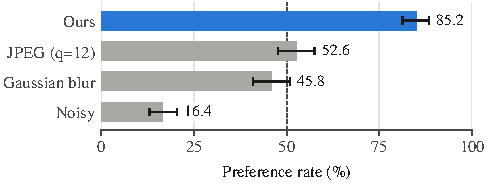
\includegraphics[width=\linewidth]{fig_preference_rate.pdf}
  \caption{User study (8 participants, 768 pairwise comparisons). TODO}
  \label{fig:preference_rate}
\end{figure}

\begin{figure}[t]
  \centering
  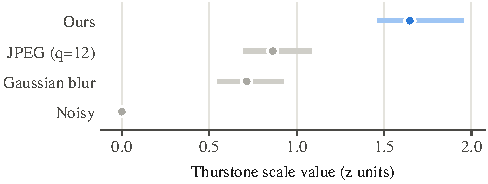
\includegraphics[width=\linewidth]{fig_scale.pdf}
  \caption{User study (8 participants, 768 pairwise comparisons). TODO}
  \label{fig:scale}
\end{figure}

\begin{figure}[t]
  \centering
  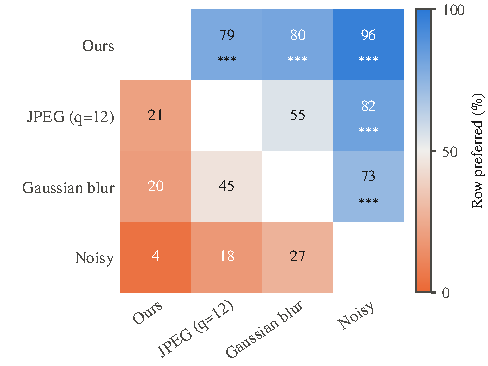
\includegraphics[width=\linewidth]{fig_pairwise.pdf}
  \caption{User study (8 participants, 768 pairwise comparisons). TODO}
  \label{fig:pairwise}
\end{figure}

\begin{figure}[t]
  \centering
  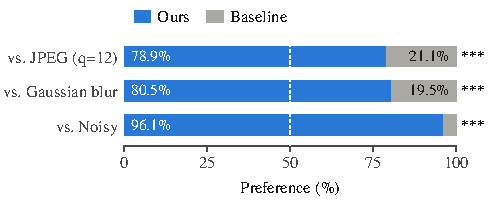
\includegraphics[width=\linewidth]{fig_ours_vs.pdf}
  \caption{User study (8 participants, 768 pairwise comparisons). TODO}
  \label{fig:ours_vs}
\end{figure}

% Double-column figure
\begin{figure*}[t]
  \centering
  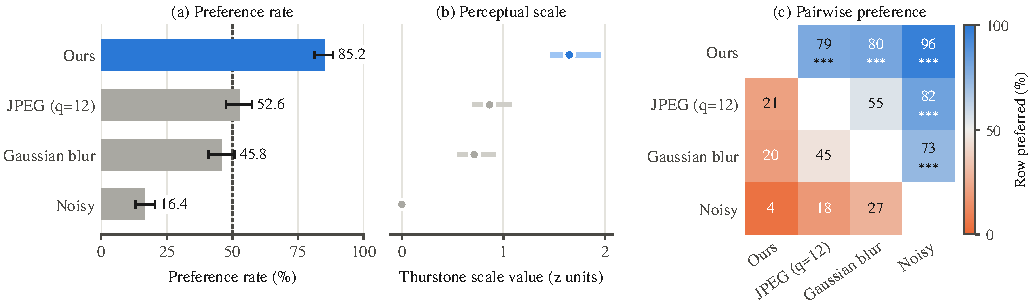
\includegraphics[width=\textwidth]{fig_overview.pdf}
  \caption{User study with 8 participants and 768 pairwise comparisons. (a) Preference rate with 95\% Wilson confidence intervals. (b) Thurstone Case~V scale values with 95\% bootstrap confidence intervals. (c) Percentage of trials in which the row method was preferred over the column method; $^{*}p<.05$, $^{**}p<.01$, $^{***}p<.001$ (two-sided binomial test, Holm-corrected).}
  \label{fig:user_study}
\end{figure*}
